% !TEX encoding = UTF-8 Unicode
% REMEMBER TO SET LANGUAGE!
\documentclass[report,12pt,norsk]{article}
\usepackage[utf8]{inputenc}
\usepackage[norsk]{babel}
% Standard stuff
\usepackage{amsmath,graphicx,varioref,verbatim,amsfonts,geometry}
% colors in text
\usepackage[usenames,dvipsnames,svgnames,table]{xcolor}
% Hyper refs
\usepackage[colorlinks]{hyperref}
\usepackage{subcaption}

% Document formatting
\setlength{\parindent}{0mm}
\setlength{\parskip}{1.5mm}

%Color scheme for listings
\usepackage{textcomp}
\definecolor{listinggray}{gray}{0.9}
\definecolor{lbcolor}{rgb}{0.9,0.9,0.9}

%Listings configuration
\usepackage{listings}
%Hvis du bruker noe annet enn python, endre det her for å få riktig highlighting.
\lstset{
	backgroundcolor=\color{lbcolor},
	tabsize=4,
	rulecolor=,
	language=python,
        basicstyle=\scriptsize,
        upquote=true,
        aboveskip={1.5\baselineskip},
        columns=fixed,
	numbers=left,
        showstringspaces=false,
        extendedchars=true,
        breaklines=true,
        prebreak = \raisebox{0ex}[0ex][0ex]{\ensuremath{\hookleftarrow}},
        frame=single,
        showtabs=false,
        showspaces=false,
        showstringspaces=false,
        identifierstyle=\ttfamily,
        keywordstyle=\color[rgb]{0,0,1},
        commentstyle=\color[rgb]{0.133,0.545,0.133},
        stringstyle=\color[rgb]{0.627,0.126,0.941}
        }
        
\newcounter{subproject}
\renewcommand{\thesubproject}{\alph{subproject}}
\newenvironment{subproj}{
\begin{description}
\item[\refstepcounter{subproject}(\thesubproject)]
}{\end{description}}

\captionsetup[subfigure]{labelformat=empty}

%Lettering instead of numbering in different layers
%\renewcommand{\labelenumi}{\alph{enumi}}
\renewcommand{\thesubsection}{\alph{subsection}}

%opening
\title{FYS1120 - Oblig 2}
\author{Joakim Flatby}

\begin{document}

\maketitle
\setcounter{section}{1}
%Oppgave 2
\section{}
 
 %a
 \subsection{)}
 $\bold{Initialverdier}$:\\
 $\vec{\bold{r}}(0) = (0,0,0)$\\
 $\vec{\bold{v}}(0) = (10$km/s$, 0, 0)$\\
 $\vec{\bold{B}} = (0,0,2T)$
 
 Plotter bevegelsen og farten komponentvis i 2D, og bevegelsen i 3D.\\
 Alt plottes over tid, fra $t = 0$ til $t=30$ps med $\Delta t = 1$fs:
 \begin{figure}[h!]
 \centering
 \begin{subfigure}{0.5\textwidth}
        	\centering 
        	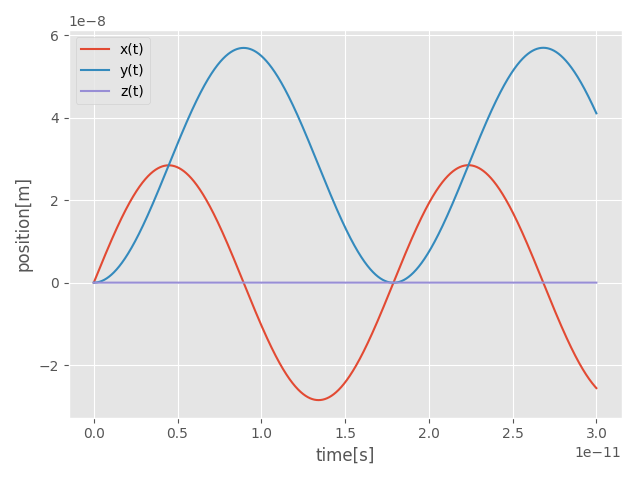
\includegraphics[width=\textwidth]{position_plot_2d.png}
       	\caption{x(t), y(t) og z(t) plottet hver for seg}
\end{subfigure}%
 \begin{subfigure}{0.5\textwidth}
        	\centering 
       	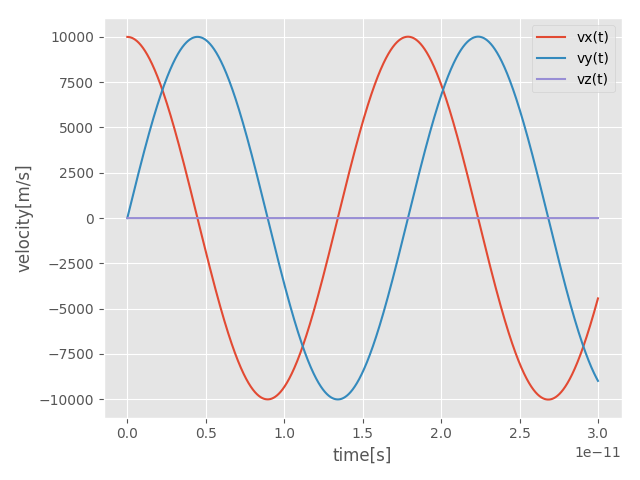
\includegraphics[width=\textwidth]{velocity_plot_2d.png}
        	\caption{$v_{x}$(t), $v_{y}$(t) og $v_{z}$(t) plottet hver for seg}
\end{subfigure}
\end{figure}

 \begin{figure}[h!]
        \centering 
        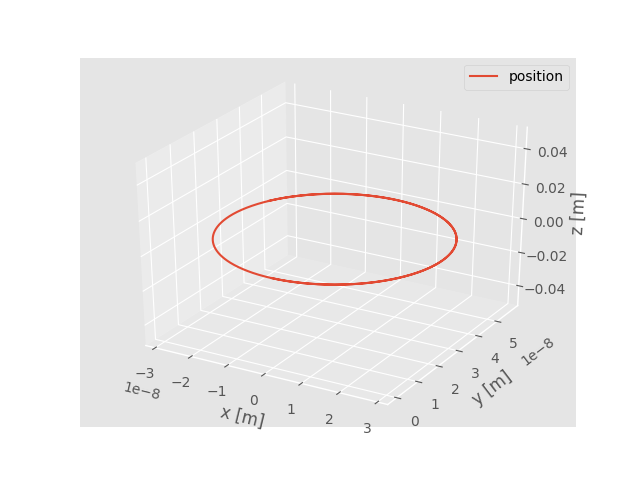
\includegraphics[scale=0.7]{position_plot_3d.png}
        \caption{Banen til partikkelen plottet i 3D}
\end{figure}

%b
\subsection{)} 
Ettersom partikkelen starter i $(0, 0, 0)$, og bare beveger seg i xy-planet, så kan jeg finne omløpstiden ved å sjekke når partikkelen er tilbake på $x\approx0$ og $y\approx0$(innenfor en viss $\epsilon$).
Etter litt prøving og feiling fant jeg $\epsilon$ som ga meg de to punktene som lå nærmest startpunktet, henholdsvis ved timestep 17887 og 17888. Ettersom disse ligger på hver sin side av $x=0$, kan jeg ta gjennomsnittet av disse, 17887.5 og gange med $dt$, som gir meg tidspunktet den kommer dit. 

Omløpstid: $t=1.78875 \cdot 10^{-11}$ s

%c
\subsection{)}

\begin{center}
Lorentz-kraften sin radielle komponent(som vil si bare den magnetiske kraften) må være lik sentripetal-kraften:

\[q \cdot v \cdot B = \frac{m \cdot v^{2}}{r}\]
$\Downarrow$
\[q \cdot B = \frac{m \cdot v}{r}\]
og ettersom $v = \omega \cdot r \Rightarrow r = \frac{v}{\omega}$, kan vi sette inn for r:
\[q \cdot B = \frac{m \cdot v \cdot \omega}{v} = m \cdot \omega\]
Løser deretter for $\omega$, og får
\[\omega = \frac{q \cdot B}{m}\]
som er det som skulle vises.

Bruker nå sammenhengen mellom vinkelfrekvens og vanlig frekvens: $\omega = 2\pi \cdot f$
$\Downarrow$
\[f = \frac{q \cdot B}{2\pi \cdot m}\]
Omløpstiden $T$ er definert som $\frac{1}{f}$, så setter inn $ f = \frac{1}{T}$
\[\frac{1}{T} = \frac{q \cdot B}{2\pi \cdot m}\]
$\Downarrow$
\[T = \frac{2\pi \cdot m}{q \cdot B}\]
\[T = \frac{2\pi \cdot (9.11 \cdot 10^{-31})}{(-1.6 \cdot 10^{-19}) \cdot 2}\]
\[T = 1.78874 \cdot 10^{-11}\]
Dette stemmer veldig bra med resultatet fra oppgave b), med bare 0.1fs forskjell.
\end{center}

%d
\subsection{)}
Kjører programmet på nytt med ny initialhastighet $v = (5000\frac{m}{s}, 0, 2000\frac{m}{s})$:
\begin{figure}[h!]
        \centering 
        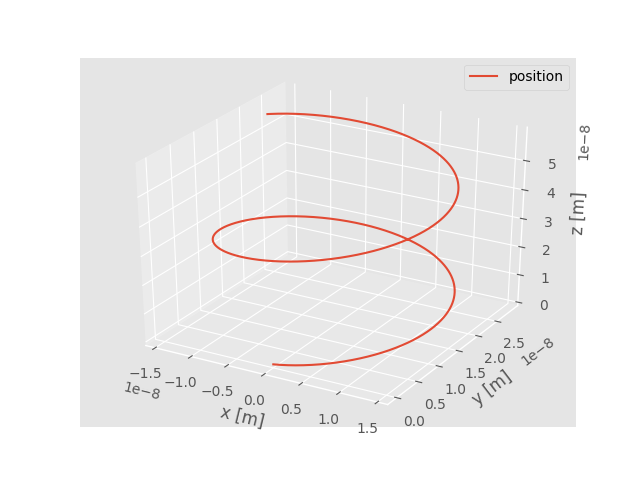
\includegraphics[scale=0.7]{position_plot_2_3d.png}
        \caption{Banen til partikkelen plottet i 3D med nye initialverdier}
\end{figure}

\newpage

\section{}
\subsection{)}

Bevegelse i $\vec{E}$- og $\vec{B}$-felt.
Gitte initialverdier med $\vec{B}$ valgt til (0, 0, 2T).

\begin{figure}[h!]
        \centering 
        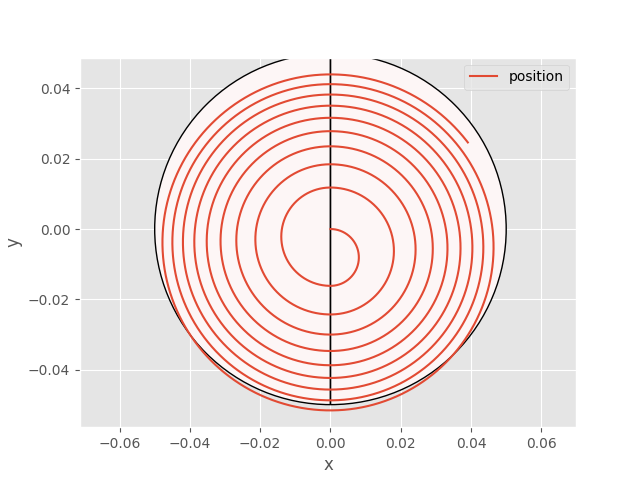
\includegraphics[scale=0.7]{cyclotron_1.png}
        \caption{Banen til et proton i en syklotron.}
\end{figure}

\newpage

Hver gang protonet passerer gjennom valley gap-et, så akselererer den i x-retning, og øker dermed samtidig radiusen i banen. Neste gang den går gjennom valley gap, har den dermed litt høyere fart enn sist gang, og vil med andre ord tilbringe kortere tid inne i valley gap-et. Dette fører til at E-feltet får kortere tid på å akselerere partikkelen hver gang, og fartsendringen(som er proporsjonal med radiusendringen), vil derfor minke for hver gang.

Man kan også se at økningen i den kinetiske energien til protonet skal være konstant og farten er proporsjonal med radiusen, så derfor må endringen i radiusen minke når farten øker:
\[E = \frac{1}{2}mv^{2}\]
\[\Delta E = mv\Delta v \propto v\Delta R\]
\newpage
\subsection{)}

\begin{figure}[h!]
 \centering
 \begin{subfigure}{0.5\textwidth}
        	\centering 
        	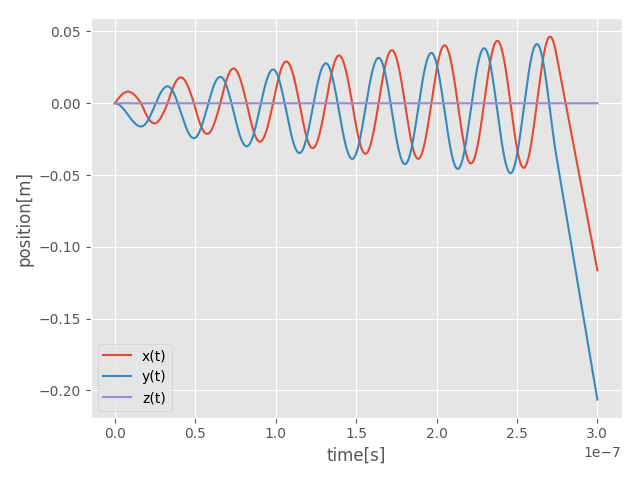
\includegraphics[width=\textwidth]{cyclotron_2.png}
       	\caption{Posisjonskomponentene over tid.}
\end{subfigure}%
 \begin{subfigure}{0.5\textwidth}
        	\centering 
       	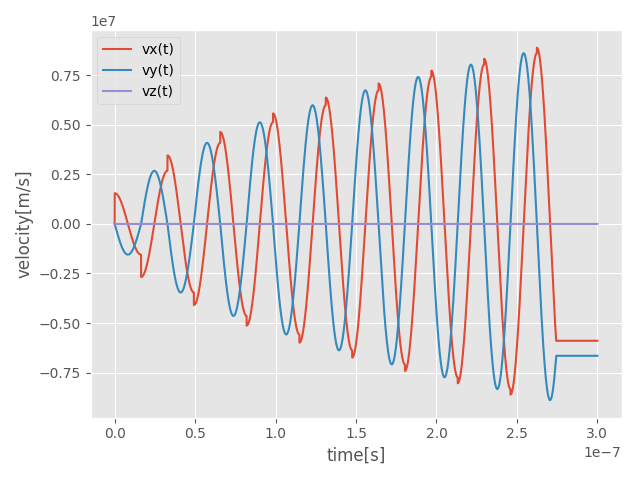
\includegraphics[width=\textwidth]{cyclotron_3.png}
        	\caption{Fartskomponentene over tid.}
\end{subfigure}
\end{figure}

\subsection{)}
Ettersom protonet har konstant fart etter å ha forlatt syklotronen, kan jeg bare printe den siste verdien til farten. (Har også dobbeltsjekket dette ved å printe farten i det time-steppet den forlater syklotronen. 

8889905.76674 $\frac{m}{s}$
Vi kan se at dette er ca. 3\% av lysfarten:
$\frac{8889905.76674}{299 792 458} = 0.0297$

\subsection{)}
\begin{center}
\[F_{B} = qvB\]
\[F_{sentripetal} = \frac{mv^{2}}{r}\]
Siden sentripetalkraften bare består av den magnetiske kraften har vi:
\[\frac{mv^{2}}{r} = qvB\]
\[\Downarrow\]
\[\frac{mv}{r} = qB\]
Ganger med r og opphøyer begge sider i 2.
\[m^{2}v^{2} = q^{2}B^{2}r^{2}\]
Hvis vi nå ganger begge sider med $\frac{1}{2m}$ får vi:
\[\frac{1}{2}mv^{2} = \frac{q^{2}B^{2}r^{2}}{2m}\]
som vil si at:
\[E_{k} = \frac{1}{2}\frac{q^{2}B^{2}r^{2}}{m}\]
\end{center}
\subsection{)}

\[E_{k} = \frac{1}{2}\frac{(1.6021766208\cdot10^{-19})^{2} \cdot 2^{2} \cdot 0.05^{2}}{1.672621898\cdot10^{-27}}\]

\[E_{k} = 7.67349 \cdot 10^{-14} J\]

Løser jeg $E_{k} = \frac{1}{2}mv^{2}$ for $v$ så får jeg $9.578833224 \cdot 10^{6} \frac{m}{s} \approx 9578833 \frac{m}{s}$

Dette stemmer ikke med det jeg fant med den ikke-relativistiske løsningen fra koden. Ettersom farten bare var 3\% av lysfarten skulle jeg ikke trodd det skulle være det relativistiske som var problemet. 

Så utifra hva jeg kan skjønne må feilmarginen komme fra den numeriske integrasjonen i koden. Jeg tenkte jeg skulle prøve å bruke leapfrog-integrasjon for å teste om det ga en fart som var nærmere den jeg får fra den analytiske løsningen, men jeg får ikke brukt leapfrog ettersom jeg da trenger akselerasjonen i [t] og [t+1] for å regne ut farten i [t+1], og for å regne ut akselerasjonen i [t+1] trenger jeg farten i [t+1]... \\

Dersom vi øker $r_{D}$ til 1 meter, så blir farten $1.915766645 \cdot 10^{8}\frac{m}{s}$, noe som er hele 64\% av lysets hastighet så her vil den ikke-relativistiske metoden definitivt bli helt feil.

\section{}
\subsection{)}

\begin{center}
Ampéres lov for $\vec{H}$-felt:
\[\int_{C}\vec{H} \cdot d\vec{l} = I\]
Symmetri gir at feltet er avhengig av $r$, men virker i $\phi$-retning:
\[\vec{H} = H(r)\hat{\phi}\]
H og l er i samme retning, så
\[\int_{C}Hdl = I\]
$\Downarrow$
\[H2\pi r = I\]
\[H = \frac{I}{2\pi r}, \text{for } a < r < b\]
ellers er $H=0$, fordi det går null netto-strøm igjennom $C$:
\[H = \begin{cases}
       \frac{I}{2\pi r}, & a < r < b\\
       0, & ellers\\
     \end{cases}\]

Bruker nå at $\vec{B} = \mu_{0} \vec{H}$ og får:

\[B = \begin{cases}
       \frac{\mu_{0} I}{2\pi r}, & a < r < b\\
       0, & ellers\\
     \end{cases}\]
     
\begin{figure}[h!]
        \centering 
        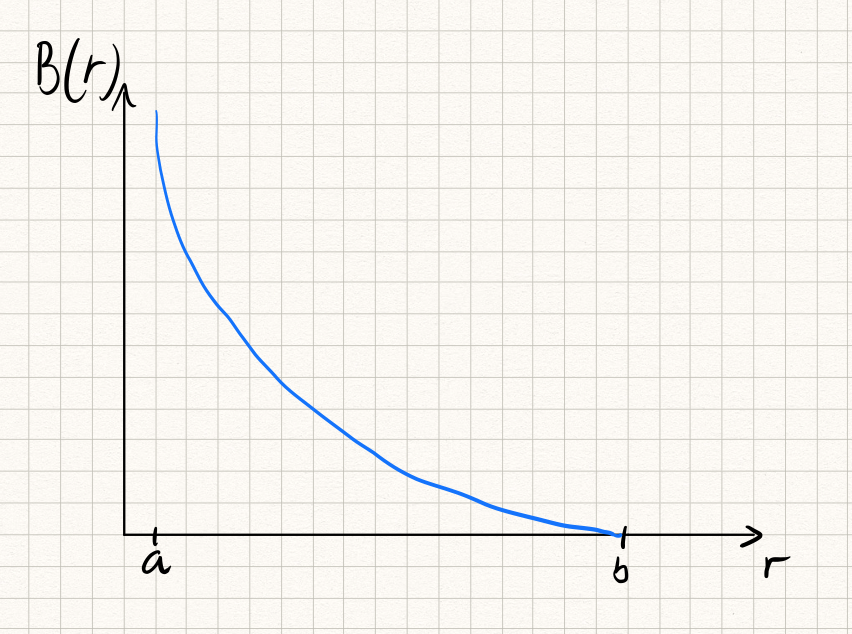
\includegraphics[scale=0.5]{koaksial_skisse.png}
        \caption{Skisse av den magnetiske feltstyrken, $|\vec{B}(r)|$}
\end{figure}
\begin{figure}[h!]
        \centering 
        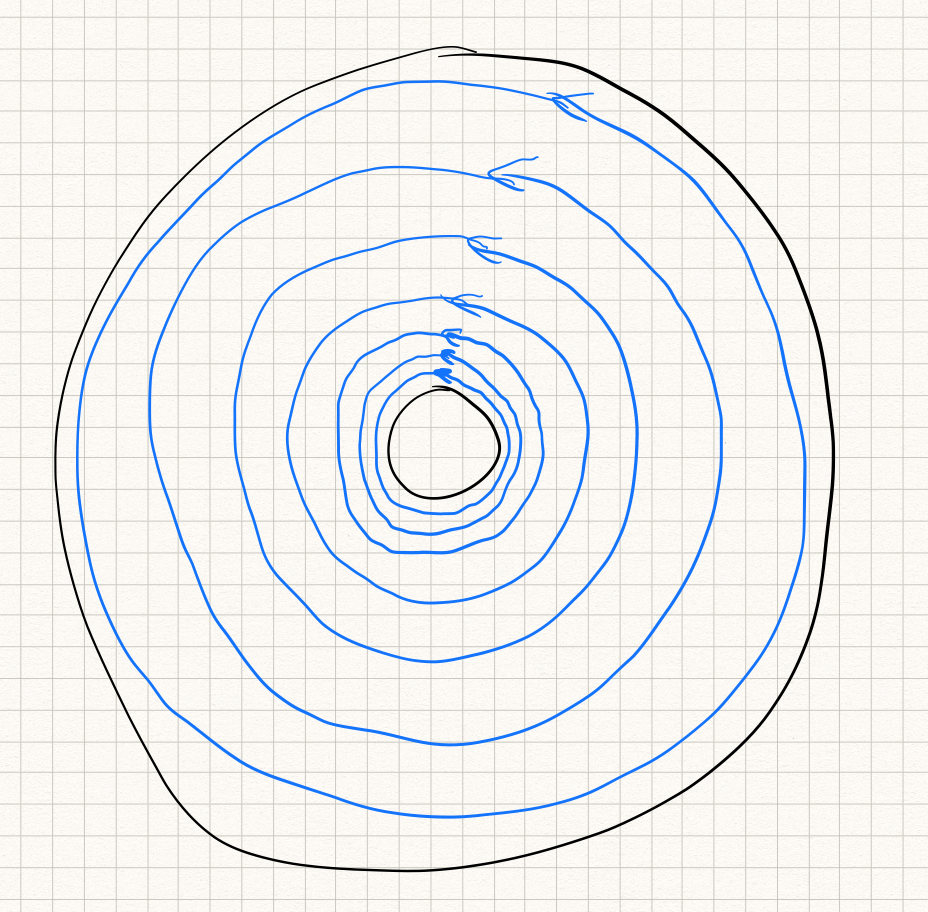
\includegraphics[scale=0.3]{koaksial_skisse2.png}
        \caption{Skisse av magnetfeltet}
\end{figure}
     
\end{center}
\newpage
\subsection{)}
Jeg tror II er den riktige skissen.

Ettersom strømmen fortsatt er jevnt fordelt utover både ytterleder og innerleder, vil begge magnetfeltene være akkurat like som før. Men siden innerlederen nå er forskjøvet, vil magnetfeltet fra denne derfor være sterkere enn magnetfeltet fra ytterlederen der avstanden er mindre, og svakere der avstanden er større. Dette fører til at magnetfeltet fra innerlederen ''stikker ut'' der innerlederen er nærmest ytterlederen, og magnetfeltet fra ytterlederen ''stikker ut'' der det er størst avstand mellom inner- og ytterleder. Akkurat som vises på skisse nr. II

\end{document}